\section{Resultados}

\begin{slide}{Análise Exploratória}
  \footnotesize
  \begin{columns}
    \begin{column}{.35\linewidth}
      \begin{Item}[0.15]
        \item Dispersão: T$_{out}$ correlacionada com entradas térmicas; fluxo com múltiplas variáveis
        \item Pearson: T$_{out}$ têm correlações lineares fortes ($|r|>0,9$); fluxo moderado ($|r|\approx0,7$)
        \item Spearman: valores próximos aos de Pearson $\rightarrow$ relações dominantes são aproximadamente lineares (monotônicas e lineares)
        \item Complexidade do fluxo $\rightarrow$ justifica modelagem multivariada
      \end{Item}
    \end{column}
    \begin{column}{.65\linewidth}
      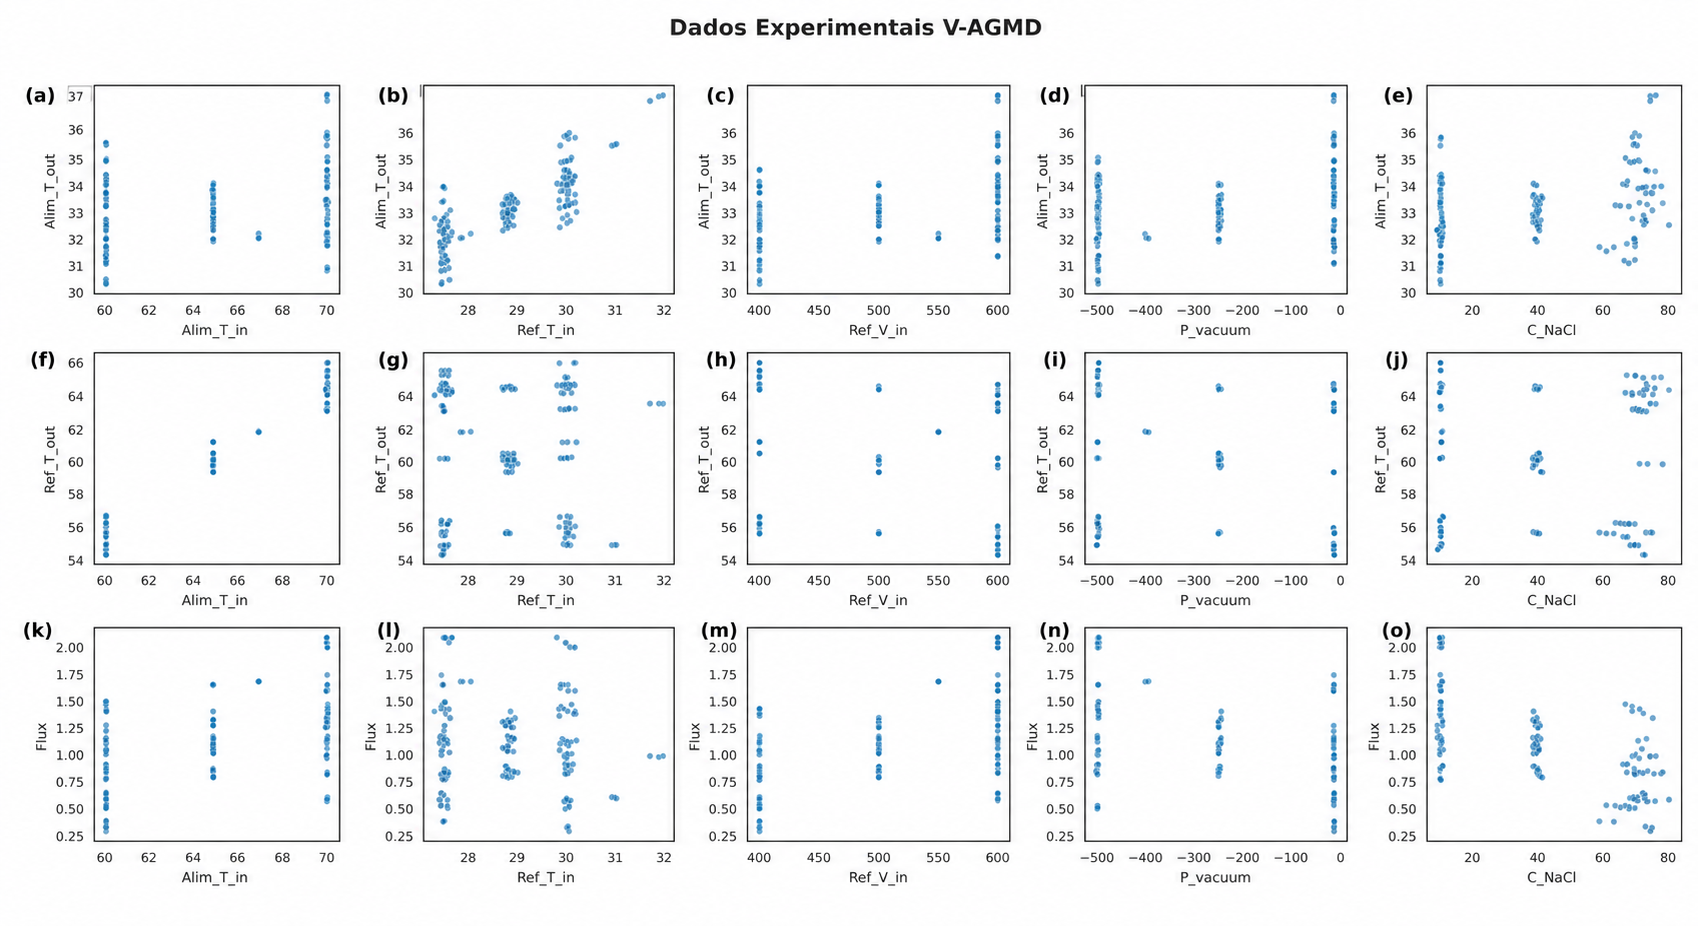
\includegraphics[width=\linewidth]{tcc_images/chap06/scatter_vagmd_exp_only.png}
    \end{column}
  \end{columns}
  \note{Análise exploratória: temperaturas de saída têm forte correlação linear (Pearson e Spearman próximos), fluxo é mais complexo. [~1 min]}
\end{slide}
%========================================================================

\begin{slide}{Modelo Físico 0D — Referência}
  \centering
  O modelo 0D de \cite{Lisboa2024} serve como referência fenomenológica para as arquiteturas híbridas. Não é um modelo desenvolvido neste trabalho.
  \vfill
  \begin{columns}
    \begin{column}{.33\linewidth}
      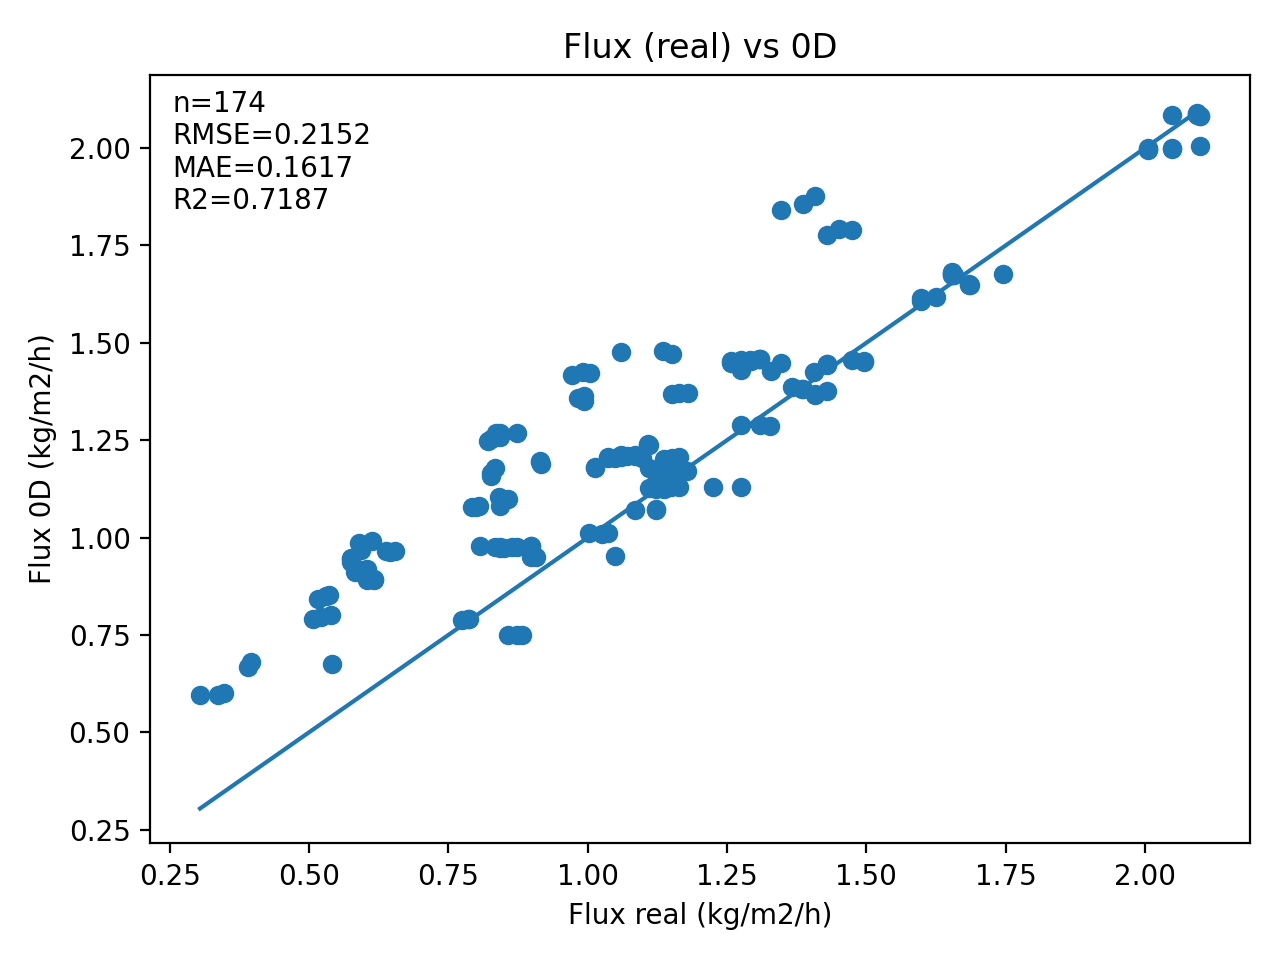
\includegraphics[width=\linewidth]{tcc_images/chap06/flux_real_vs_0d.png}
    \end{column}
    \begin{column}{.33\linewidth}
      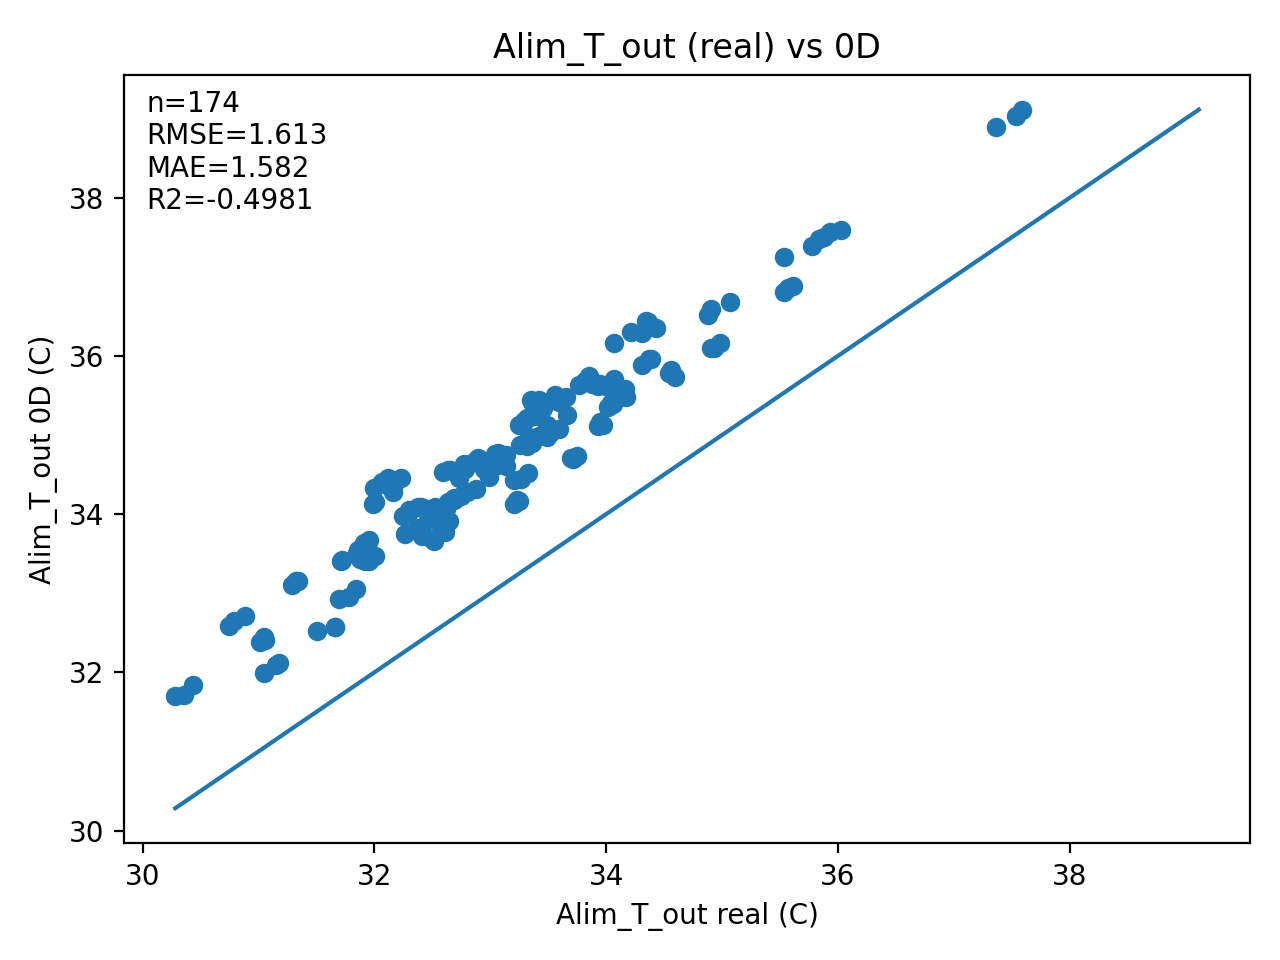
\includegraphics[width=\linewidth]{tcc_images/chap06/alim_T_out_real_vs_0d.png}
    \end{column}
    \begin{column}{.33\linewidth}
      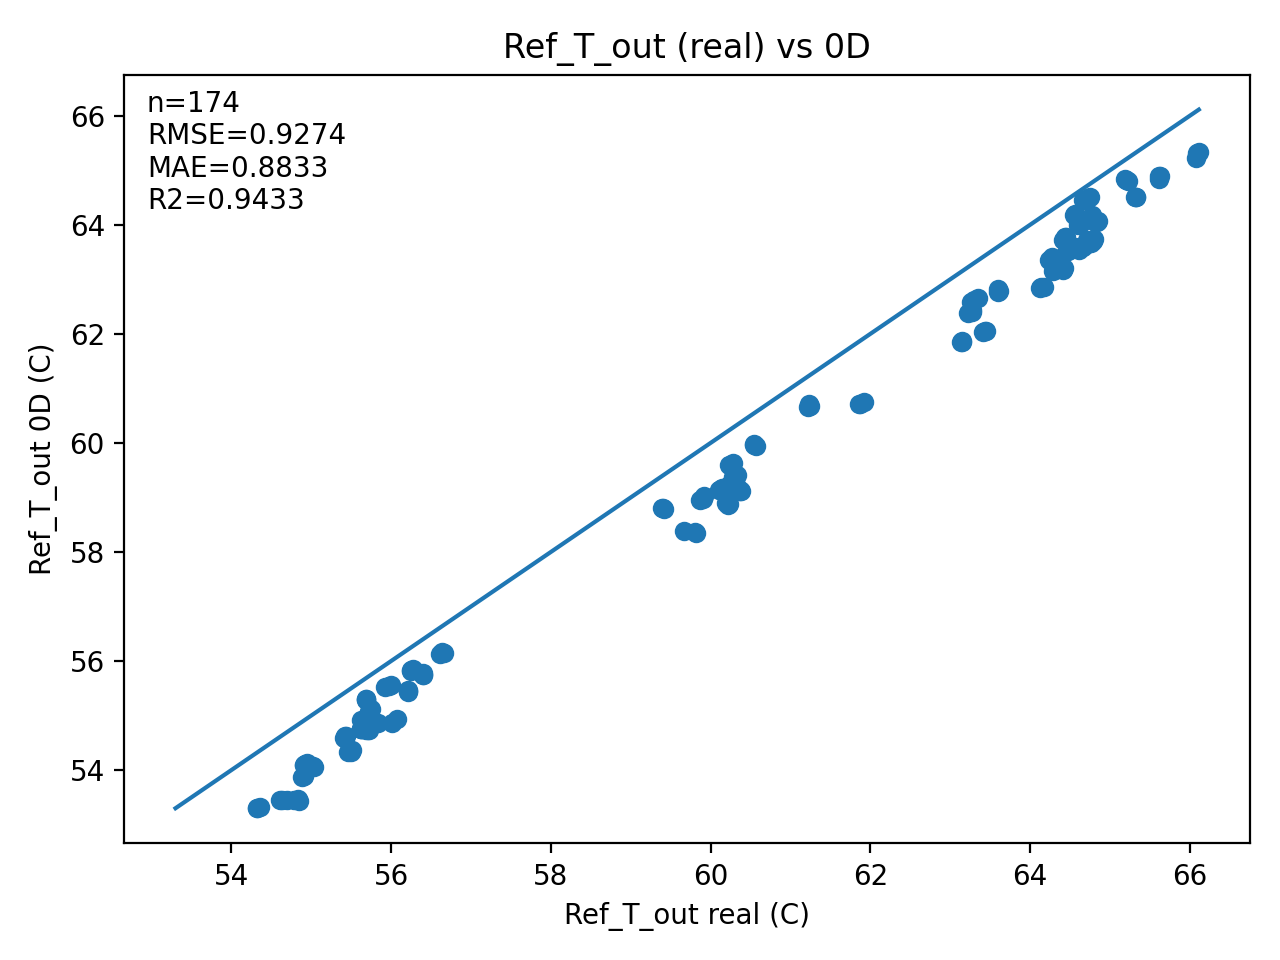
\includegraphics[width=\linewidth]{tcc_images/chap06/ref_T_out_real_vs_0d.png}
    \end{column}
  \end{columns}
  \vfill
  {\scriptsize Predição do modelo 0D \textit{vs} experimental para cada variável de saída. Modelo 0D: \cite{Lisboa2024}}
  \note{O modelo 0D de Lisboa et al. (2024) é a referência física — não é um modelo desenvolvido neste trabalho. As arquiteturas híbridas aprendem a corrigir sistematicamente suas predições a partir dos dados experimentais. [~30s]}
\end{slide}
%========================================================================

% Tabela detalhada removida a pedido da orientadora (S30-S34): manter apenas a tabela consolidada
% \begin{slide}{Stage 0 — Modelos Lineares}
%   ... (conteúdo movido para o material suplementar)
% \end{slide}

\begin{slide}{Stage 0 — Modelos Lineares e Árvores}
  \centering
  \small
  \textbf{Modelos lineares} (OLS, Ridge, Lasso, ElasticNet): desempenho similar entre si; regularização não trouxe ganho significativo sobre OLS.
  \vfill
  \textbf{Árvores de decisão} (DT, RF, GB): DT e RF overfitam nos regimes de treino (CV alto); GB generaliza melhor, mas ainda inferior aos lineares.
  \vfill
  {\scriptsize Detalhes das tabelas de Stage 0 no material suplementar.}
  \note{Stage 0: lineares — OLS, Ridge, Lasso, ElasticNet têm desempenho similar. Árvores — DT e RF overfitam; GB generaliza melhor mas inferior aos lineares. [~1 min]}
\end{slide}
%========================================================================

% Tabela detalhada removida a pedido da orientadora (S30-S34): manter apenas a tabela consolidada
% \begin{slide}{Stage 0 — Árvores de Decisão}
%   ... (conteúdo movido para o material suplementar)
% \end{slide}
%========================================================================

\begin{slide}{Stage 1 — Redes Neurais}
  \centering
  \scriptsize
  \begin{tabular}{llcccccc}
    \toprule
    \textbf{Arquitetura} & \textbf{Alvo} & \multicolumn{3}{c}{\textbf{CV RMSE}} & \multicolumn{3}{c}{\textbf{Test RMSE}} \\
    \cmidrule(lr){3-5} \cmidrule(lr){6-8}
    & & T$_{alim}$ & T$_{ref}$ & Flux & T$_{alim}$ & T$_{ref}$ & Flux \\
    \midrule
    (128,64), tanh, lr=0,001, l2=0,001 & Alim & 0,260 & \textbf{0,445} & 0,115 & 0,215 & \cellcolor{orange!10}\textbf{0,309} & 0,073 \\
    (128,64), tanh, lr=0,001, l2=0,001 & Ref & 0,267 & 0,459 & 0,116 & 0,227 & 0,318 & 0,073 \\
    (128,64,32), relu, lr=0,003, l2=0,0 & Flux & \textbf{0,222} & 0,554 & \textbf{0,081} & \cellcolor{blue!10}\textbf{0,178} & 0,369 & \cellcolor{green!10}\textbf{0,066} \\
    \bottomrule
  \end{tabular}
  \note{Três baselines de redes neurais. A otimizada para Flux tem arquitetura maior (128,64,32) mas L2=0. [~1 min]}
\end{slide}
%========================================================================

\begin{slide}{Stage 2 — Modelos Híbridos}
  \centering
  \scriptsize
  \begin{tabular}{llcccccc}
    \toprule
    \textbf{Modelo} & \textbf{Alvo} & \multicolumn{3}{c}{\textbf{CV RMSE}} & \multicolumn{3}{c}{\textbf{Test RMSE}} \\
    \cmidrule(lr){3-5} \cmidrule(lr){6-8}
    & & T$_{alim}$ & T$_{ref}$ & Flux & T$_{alim}$ & T$_{ref}$ & Flux \\
    \midrule
    \textbf{PhyResidual} & \textbf{Alim} & 0,275 & \textbf{0,301} & \textbf{0,060} & 0,225 & 0,222 & 0,057 \\
    \textbf{PhyResidual} & \textbf{Ref} & 0,274 & 0,305 & 0,061 & 0,224 & 0,231 & 0,058 \\
    \rowcolor{green!6}
    \textbf{PhyResidual} & \textbf{Flux} & \textbf{0,236} & 0,346 & 0,072 & \cellcolor{blue!10}\textbf{0,183} & \cellcolor{orange!10}\textbf{0,214} & \cellcolor{green!10}\textbf{0,054} \\
    PhyHybrid & Alim & 0,273 & 0,306 & 0,061 & 0,224 & 0,231 & 0,058 \\
    PhyHybrid & Ref & 0,275 & 0,302 & 0,061 & 0,225 & 0,230 & 0,058 \\
    PhyHybrid & Flux & 0,284 & 0,399 & 0,075 & 0,222 & 0,239 & 0,055 \\
    PhyInput & Alim & 0,273 & 0,325 & 0,098 & 0,213 & 0,250 & 0,064 \\
    PhyInput & Ref & 0,275 & 0,432 & 0,106 & 0,216 & 0,269 & 0,066 \\
    PhyInput & Flux & 0,260 & 0,625 & 0,104 & 0,213 & 0,426 & 0,063 \\
    \midrule
    PhyLoss ($\omega{=}0{,}0$) & Alim & 0,180 & 0,348 & 0,067 & 0,188 & 0,350 & 0,068 \\
    PhyLoss ($\omega{=}0{,}7$) & Ref  & 0,310 & 0,276 & 0,192 & 0,340 & 0,286 & 0,220 \\
    PhyLoss ($\omega{=}0{,}0$) & Flux & 0,203 & 0,422 & 0,066 & 0,226 & 0,438 & 0,069 \\
    \bottomrule
  \end{tabular}
  \note{PhyResidual (base Flux) teve o menor Test RMSE nos três alvos entre os híbridos. Para T\_ref, diferença sobre Ridge é marginal (2,3\%); Ridge tem melhor CV (extrapolação). [~2 min]}
\end{slide}
%========================================================================

\begin{slide}{Comparação Final — Consolidado por Variável de Saída}
  \centering
  \footnotesize
    \begin{tabular}{lclcccc}
    \toprule
    \textbf{Variável de saída} & \textbf{Estágio} & \textbf{Modelo} & \textbf{Test RMSE} & \textbf{CV RMSE} & \textbf{Test R$^2$} \\
    \midrule
    \textbf{T$_{alim,out}$} & Stage 0 & OLS & 0,231 & \textbf{0,196} & 0,965 \\
    \textbf{T$_{alim,out}$} & Stage 1 & Baseline Flux & \textbf{0,178} & 0,081 & 0,981 \\
    \textbf{T$_{alim,out}$} & Stage 2 & PhyResidual (Flux) & 0,183 & 0,275 & 0,981 \\
    \midrule
    \textbf{T$_{ref,out}$} & Stage 0 & Ridge (Ref) & 0,219 & \cellcolor{yellow!15}\textbf{0,244} & 0,996 \\
    \textbf{T$_{ref,out}$} & Stage 1 & Baseline Alim & 0,309 & 0,445 & 0,989 \\
    \textbf{T$_{ref,out}$} & Stage 2 & PhyResidual (Flux) & \textbf{0,214} & 0,346 & \textbf{0,996} \\
    \midrule
    \textbf{Flux} & Stage 0 & Lasso (Flux) & 0,075 & 0,082 & 0,951 \\
    \textbf{Flux} & Stage 1 & Baseline Flux & 0,066 & 0,081 & 0,972 \\
    \textbf{Flux} & Stage 2 & PhyResidual (Flux) & \textbf{0,054} & \textbf{0,072} & \textbf{0,979} \\
    \midrule
    \rowcolor{gray!6}
    \textbf{Flux} & \multirow{3}{*}{\textbf{Modelo 0D}} & --- & 0,206 & --- & 0,631 \\
    \rowcolor{gray!6}
    \textbf{T$_{alim,out}$} & & --- & 1,549 & --- & $-$0,404 \\
    \rowcolor{gray!6}
    \textbf{T$_{ref,out}$} & & --- & 0,851 & --- & 0,948 \\
    \bottomrule
  \end{tabular}
  \note{Test RMSE em negrito = menor erro por variável; CV RMSE em negrito = melhor generalização. O Flux foi a única saída onde o menor Test RMSE e o menor CV RMSE pertencem ao mesmo modelo. [~2 min]}
\end{slide}
%========================================================================

\begin{slide}{Predição vs Experimental — Modelos Selecionados}
  \centering
  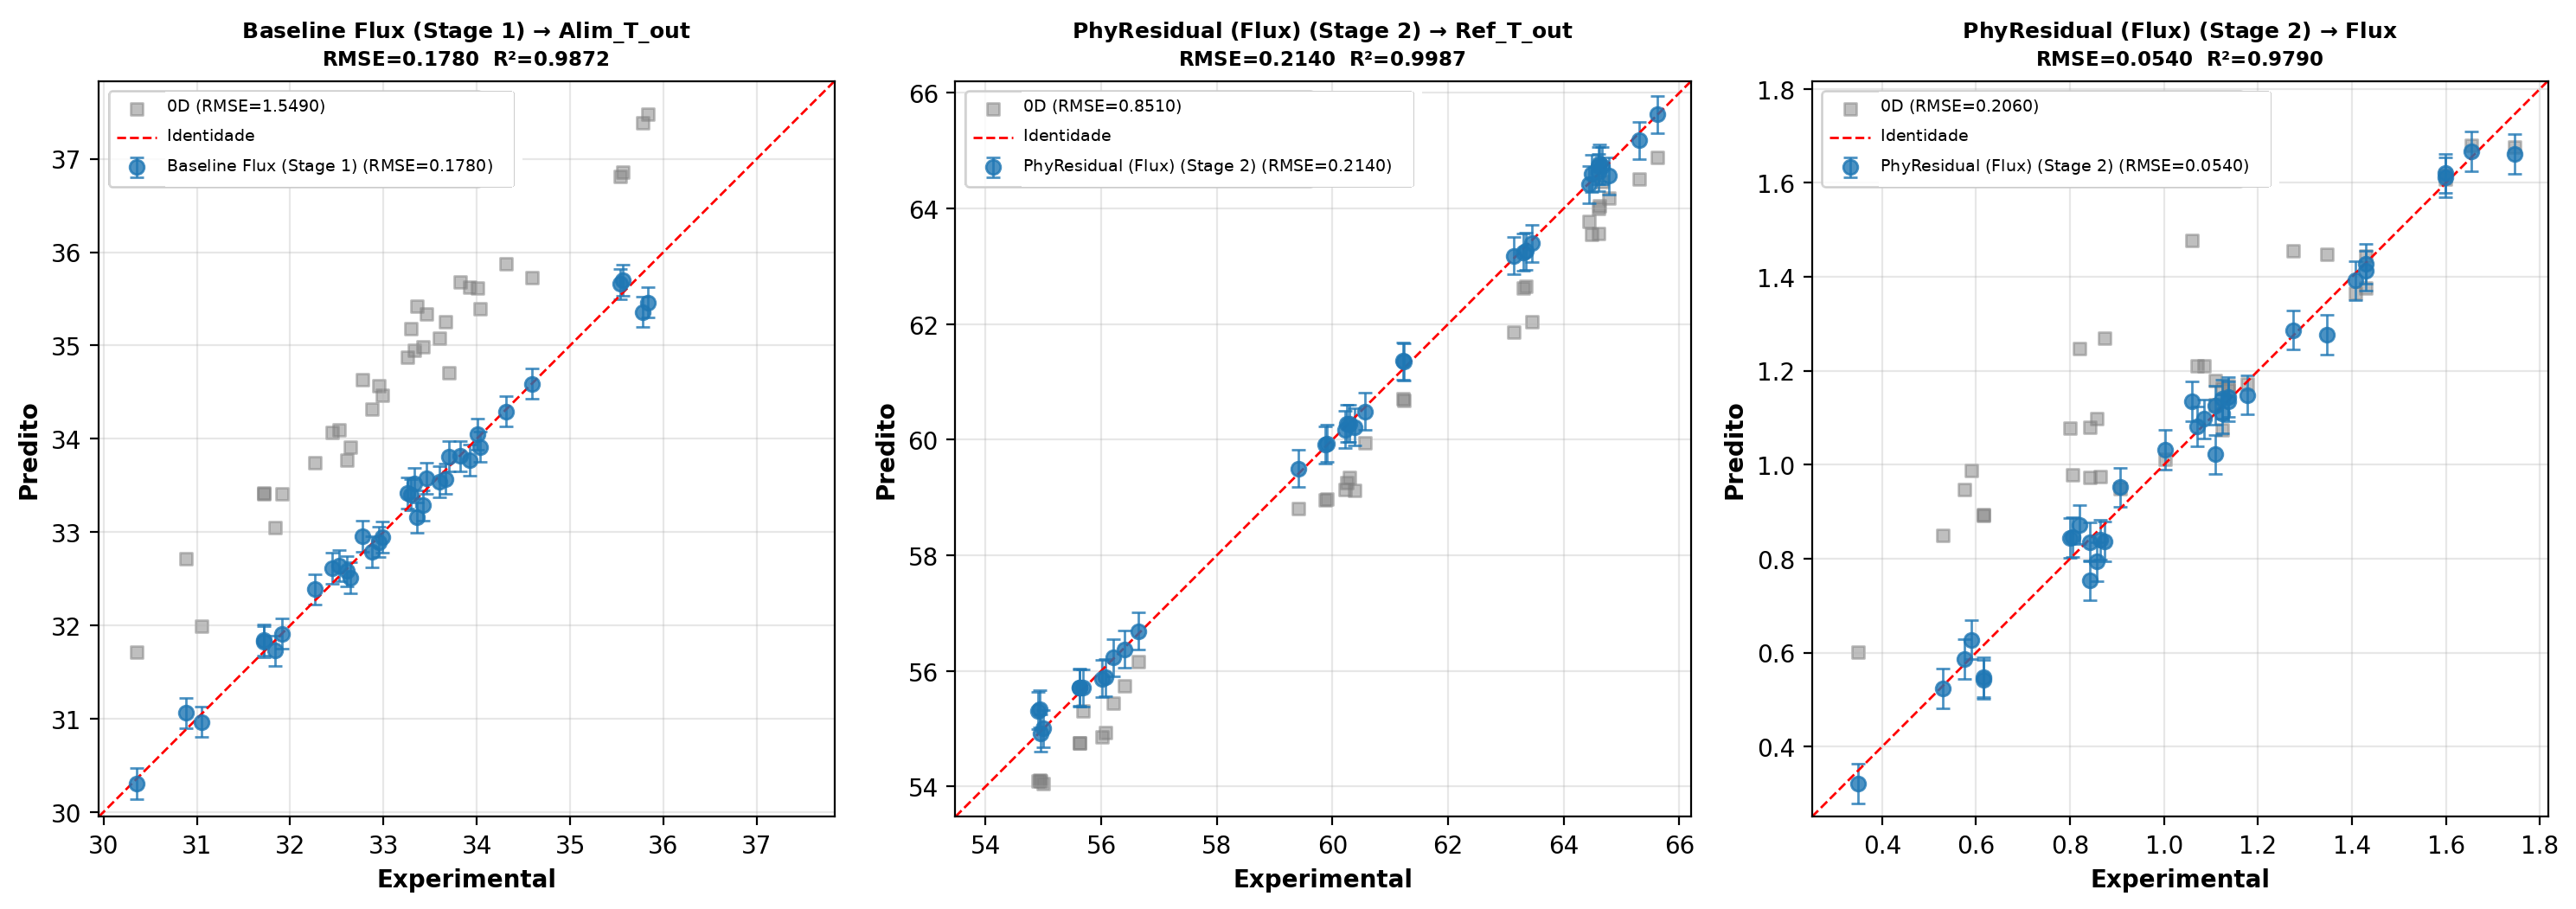
\includegraphics[width=0.85\textwidth]{tcc_images/chap06/model_selection/overlay_champions_panel_v2.png} b
  \vfill
    {\scriptsize \textcolor{blue!70!black}{T$_{alim,out}$}: Baseline Flux (Stage 1) \;|\;
    \textcolor{orange!70!black}{T$_{ref,out}$}: PhyResidual$^{Flux}$ (Stage 2) \;|\;
    \textcolor{green!70!black}{Flux}: PhyResidual$^{Flux}$ (Stage 2)}
  \\
  {\scriptsize Quadrados cinza = modelo físico 0D}
  \note{Overlay com os modelos selecionados: Baseline Flux para T\_alim (Stage 1), PhyResidual (base Flux) para T\_ref e Flux (Stage 2). Quadrados cinza = modelo 0D. [~1 min]}
\end{slide}
%========================================================================
